\section{绝对值函数}
\begin{definition}[绝对值]
设\(x \in \mathbb{R}\),则称函数\begin{equation*}
	f(x) = \left\{ \begin{array}{c}
		x, \quad x \geq 0 \\
		-x, \quad x < 0
	\end{array} \right.
\end{equation*}为\(x\)的绝对值,
记作\(\abs{x}\).
\end{definition}

\begin{figure}[htb]
	\centering
	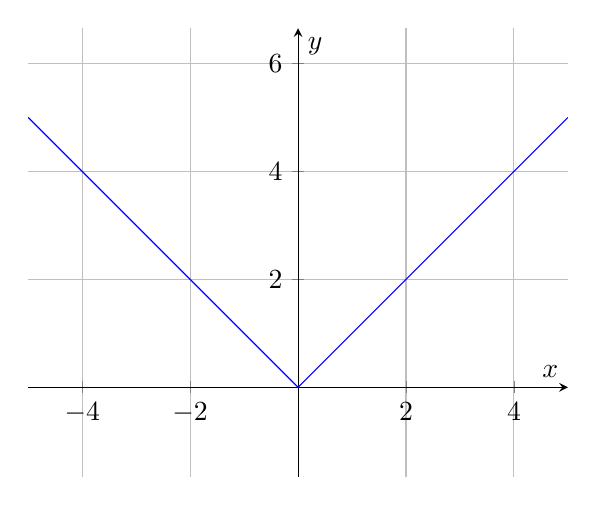
\begin{tikzpicture}
		\begin{axis}[
			xmin=-5,xmax=5,
			ymin=0,ymax=5,
			grid=both,
			axis lines=middle,
			xlabel=$x$,
			ylabel=$y$,
			axis equal=true,
		]
			\addplot[color=blue,samples at={-5,0,5}]{abs(x)};
		\end{axis}
	\end{tikzpicture}
	\caption{绝对值函数\(\abs{x}\)的图形}
\end{figure}

\begin{proposition}
设\(a,b\in\mathbb{R}\),
则\begin{itemize}
	\item \(\abs{a}\geq0\),
	\item \(\abs{a} = \abs{-a}\),
	\item \(\abs{ab} = \abs{a} \abs{b}\),
	\item \(\abs{\frac{a}{b}} = \frac{\abs{a}}{\abs{b}}\ (b\neq0)\),
	\item \(\abs{a}^2 = \abs{a^2}\).
\end{itemize}
\begin{proof}
当\(a=0\)或\(b=0\)时,易见\(\abs{ab} = 0 = \abs{a} \abs{b}\).
当\(a\neq0\)且\(b\neq0\)时,
按照\(a\)和\(b\)的不同取值,列表如下:
\begin{center}
	\begin{tblr}{|*2c|*2{c|}}
		\hline
		&& \(b>0\) & \(b<0\) \\
		&& \(\abs{b}=b\) & \(\abs{b}=-b\) \\ \hline
		\(a>0\) & \(\abs{a}=a\) & \(ab>0,\abs{ab}=ab\) & \(ab<0,\abs{ab}=-ab\) \\ \hline
		\(a<0\) & \(\abs{a}=-a\) & \(ab<0,\abs{ab}=-ab\) & \(ab>0,\abs{ab}=ab\) \\ \hline
	\end{tblr}
\end{center}
由此可知\(\abs{ab} = \abs{a} \abs{b}\)恒成立.
\end{proof}
\end{proposition}

\begin{proposition}
设\(a\)和\(b\)都是实数,
则\begin{gather}
	\min\{a,b\}
	= \frac{a+b}{2}
	- \frac{\abs{a-b}}{2},
		\label{equation:绝对值函数.两个数的最小值} \\
	\max\{a,b\}
	= \frac{a+b}{2}
	+ \frac{\abs{a-b}}{2}.
		\label{equation:绝对值函数.两个数的最大值}
\end{gather}
\begin{proof}
当\(a>b\)时,有\begin{equation*}
	\frac{a+b}{2} - \frac{\abs{a-b}}{2}
	= \frac{a+b}{2} - \frac{a-b}{2}
	= \frac{2b}{2} = b
	= \min\{a,b\},
\end{equation*}\begin{equation*}
	\frac{a+b}{2} + \frac{\abs{a-b}}{2}
	= \frac{a+b}{2} + \frac{a-b}{2}
	= \frac{2a}{2} = a
	= \max\{a,b\}.
\end{equation*}
当\(a \leq b\)时,有\begin{equation*}
	\frac{a+b}{2} - \frac{\abs{a-b}}{2}
	= \frac{a+b}{2} - \frac{b-a}{2}
	= \frac{2a}{2} = a
	= \min\{a,b\},
\end{equation*}\begin{equation*}
	\frac{a+b}{2} + \frac{\abs{a-b}}{2}
	= \frac{a+b}{2} + \frac{b-a}{2}
	= \frac{2b}{2} = b
	= \max\{a,b\}.
	\qedhere
\end{equation*}
\end{proof}
\end{proposition}

\begin{corollary}
设\(a\)和\(b\)都是实数,
则\begin{equation}
	\max\{a,b\} + \min\{a,b\} = a + b.
		\label{equation:绝对值函数.两个数的最小值最大值的关联}
\end{equation}
\begin{proof}
将\cref{equation:绝对值函数.两个数的最小值,equation:绝对值函数.两个数的最大值}
相加便得.
\end{proof}
\end{corollary}
